% !TeX root = ../main.tex

\chapter{Evaluation}\label{chapter:evaluation}
To verify the capability of the approach proposed in this work, the prototypical implementation was tested.
The idea is to find out, whether the approach is capable of detecting copied code in a codebase and, by that, unveil license infringements.
For that purpose, 2000 GPL licensed projects were indexed using the prototypical implementation of the tool.
After that, other open source projects, which are licensed not compatible with GPL and therefore should not contain any GPL licensed code indexed before, where analyzed and emerging matches categorized.

This chapter describes the test setup evaluates timings, database sizes and findings.

\section{Test Setup}
As a source for the projects to index, GitHub was chosen.
GitHub's REST API was used to generate a list of 1.000 GPL licensed Java and 1.000 GPL licensed C or C++ projects.
All of the projects were checked out locally resulting in sizes as shown in \autoref{table:locs}.

Indexing those 2.000 projects including their history took 16h on a consumer laptop with 16 GB of RAM and an Intel i7 2.6 GHz CPU with 4 cores and hyper-threading.
The indexing was done independently for Java and C/C++ generating two databases.
The resulting database sizes are 4 GB for Java and 33 GB for C/C++, the bloom filter's sizes are 55 MB and 147 MB for Java and C/C++.

Inspection of several indexed projects showed, the huge difference fo the sizes can be justified in the amount of actual code in the repositories.
It seems like Java projects contain more images, binary files or other resources, compared to the C/C++ projects.

\begin{table}[ht]
	\centering
	\begin{tabular}{l|rrrrr}
		& \textbf{Scanned Files} & \textbf{Lines of Code} & \textbf{Total size} & \textbf{Hashes} & \textbf{Chunks} \\ 
		\hline 
		Java & 836.555 & 57.834.764 & 94 GB & 23.773.065 & 35.069.633 \\
		C/C++ & 1.023.092 & 380.338.327 & 102 GB & 61.349.163 & 221.315.454 \\ 
	\end{tabular}
	\caption{Sizes of the 2.000 indexed projects}\label{table:locs}
\end{table}

After two weeks, the index was updated for both Java and C/C++ as described in \ref{section:implementation/history_analysis/update}.
Approximately one third of the reference projects contained one or more new tags which were indexed.
The update took a total of one hour including calculation of the bloom filter.
This shows that incremental updates of the index are worth the effort of implementation compared to re-indexing the reference projects from scratch.

After indexing those projects, several other projects, licensed not compatible with GPL, where analyzed for matches using the approach described in section \ref{section:implementation/finding_matches}.
\autoref{table:target_projects} shows the chosen target projects, their license and the lines of code of files written in the corresponding language.

\todo{Exclude third party and generated code}

\begin{table}[ht]
	\centering
	\begin{tabular}{l|llr}
		& \textbf{Name} & \textbf{License} & \textbf{Lines of Code} \\
		\hline 
		\parbox[t]{2mm}{\multirow{12}{*}{\rotatebox[origin=c]{90}{JAVA}}} 
		& IntelliJ IDEA Community & Apache 2.0 & 3.500.000 \\
		& Eclipse JDT Core & Eclipse Public License & 1.459.000 \\
		& Elasticsearch & Apache 2.0 & 711.000 \\
		& Eclipse JDT UI & Eclipse Public License & 685.000 \\
		& Facebook Buck & Apache 2.0 & 597.000 \\
		& Teamscale & Closed Source & 480.000 \\
		& Spring Boot & Apache 2.0 & 223.000 \\
		& Openfire & Apache 2.0 & 200.000 \\
		& Killbill & Apache 2.0 & 150.000 \\
		& JabRef & MIT & 125.000 \\
		& Selenium & Apache 2.0 & 84.000 \\
		& JUnit5 & Apache 2.0/Eclipse Public License & 45.000 \\
		\hline 
		\parbox[t]{2mm}{\multirow{10}{*}{\rotatebox[origin=c]{90}{C/C++}}} 
		& Chromium & BSD License 2.0 & 4.651.000 \\
		& ArangoDB & Apache 2.0 & 4.855.000 \\
		& Tensorflow & Apache 2.0 & 662.000 \\
		& Apple Swift & Apache 2.0 & 520.000 \\
		& Mesos & Apache 2.0 & 309.000 \\
		& Apache httpd & Apache 2.0 & 214.000 \\
		& RethinkDB & Apache 2.0 & 201.000 \\
		& Tesseract & Apache 2.0 & 147.000 \\
		& Bitcoin & MIT & 119.000 \\
		& Electron & MIT & 67.000 \\
	\end{tabular}
	\caption{Target projects used for testing, their license and LOCs in the corresponding language}\label{table:target_projects}
\end{table}


\section{Hash Filter Performance}\label{section:evaluation/findings/hash_filter_performance}
The bloom filter can return false positives, thus, matches are expected even if no code has been copied from a reference project into the target project for large enough projects.
Those matches - called false positive filter matches (FPFM) \todo{FPFM needed?} in the remainder of this work - are expected to occur once for roughly every 10.000 statements in the target project, since the probability for a false positive of the bloom filter is calculated to be 0,01\%. 

Table \autoref{table:unfiltered_findings} lists results regarding amount of analyzed chunks as well as false and true positive matches.
The first two colums called \textit{Files} and \textit{Chunks} show the amount of scanned files and the resulting number of chunks extracted from the target system.
The FPFMs and the percentage in relation to all matches are shown in the third column.
The last column shows the amount of actual matches, which could be found in the index and their relative amount in comparison to all chunks extracted from the target system.
\todo{more details on match distribution and assertions about significance}

\begin{table}[ht]
	\centering
	\begin{tabular}{l|lrrrr}
		 & \textbf{Target System} & \textbf{Files} & \textbf{Chunks} & \textbf{False Positives} & \textbf{True Positives} \\ 
		\hline 
		\parbox[t]{2mm}{\multirow{12}{*}{\rotatebox[origin=c]{90}{JAVA}}} 
		& IntelliJ IDEA Community & 0 & 0 & 0 & 0 \\
		& Eclipse JDT Core & 0 & 0 & 0 & 0  \\
		& Elasticsearch & 0 & 0 & 0 & 0  \\
		& Eclipse JDT UI & 0 & 0 & 0 & 0  \\
		& Facebook Buck & 0 & 0 & 0 & 0  \\
		& Teamscale & 0 & 0 & 0 & 0  \\
		& Spring Boot & 0 & 0 & 0 & 0 \\
		& Openfire & 0 & 0 & 0 & 0  \\
		& Killbill & 0 & 0 & 0 & 0  \\
		& JabRef & 0 & 0 & 0 & 0 \\
		& Selenium & 0 & 0 & 0 & 0 \\
		& JUnit5 & 0 & 0 & 0 & 0 \\
		\hline 
		\parbox[t]{2mm}{\multirow{10}{*}{\rotatebox[origin=c]{90}{C/C++}}} 
		& Chromium & 0 & 0 & 0 & 0 \\
		& ArangoDB & 0 & 0 & 0 & 0 \\
		& Tensorflow & 0 & 0 & 0 & 0 \\
		& Apple Swift & 0 & 0 & 0 & 0 \\
		& Mesos & 0 & 0 & 0 & 0 \\
		& Apache httpd & 0 & 0 & 0 & 0 \\
		& RethinkDB & 0 & 0 & 0 & 0 \\
		& Tesseract & 0 & 0 & 0 & 0 \\
		& Bitcoin & 0 & 0 & 0 & 0 \\
		& Electron & 0 & 0 & 0 & 0 \\
	\end{tabular}
	\caption{Amount of files and chunks as well as true and false positives caused by the Hash Filter}\label{table:unfiltered_findings}
\end{table}

This result shows, that the Hash Filter is reducing the required lookups by TODO in the worst case.
Load on the server can be greatly reduced and analysis of a target system's code is a lot quicker.
Still, requesting the locations for each hash passing the Hash Filter individually, causes a lot of requests with high overhead caused by creating single network packets.
Additional authentication on the server may be required to control access further slowing down the analysis.
Instead, sending hashes in batches may be a better solution.

\section{Detection of License Infringements}
As the previous section shows, matches have to be filtered, in order to remove false positives and matches, which are not relevant in the context of license infringement.
Aggregation and filtering is done as described in \autoref{section:implementation/finding_matches}.

To get a better view on the results, they are grouped into three categories:
\begin{description}
	\item [Accidential Clones (AC)]
		Matches which are similar by \glqq accident\grqq, e.g. generated code, interface implementations, declarations of structs/enums, switch-case blocks, table data especially present in C/C++.
	\item[Otherwise Licensed Code (OLC)]
		Code which is actually copied, sometimes from a common source and therefore is no direct license infringement.
		This can be relevant nonetheless, since attribution has to be done correctly, see later this section.
		Code can also be copied into the reverse direction in the context of this evaluation, since analyzed target projects are licensed in a way, where they can be copied to GPL licensed code with appropriate attribution.
	\item[License Infringement (LI)]
		Code which has been copied and is violating the license of the reference system.
\end{description}

A scanned target system file can have multiple matches for a chunk, since clones also exist between and within reference systems.
Therefore, in the following evaluation, matches are counted on the target file and only the most relevant concatenated matches of the reference files are regarded.
\autoref{table:scan_results} shows the results of manually categorizing each match.
A match is a relation between a file of the target system to the best match of a file in a reference system, indicating a high similarity.

If a target file has multiple sections of copied code, which \textit{does not overlap} and is from multiple other files (e.g. common in utils code), each match in the target file is counted once.
Figure \ref{fig:match_counting} shows an example, where multiple sections of code are copied from \texttt{Reference File 1} to the \texttt{Target File}.
This is counted as one match.
There is also one coherent block of code copied from \texttt{Reference File 2} to the \texttt{Target File}, which is also counted as a match.
The resulting total count of matches for the \texttt{Target File} in this example is two.

\begin{figure}
	\centering
	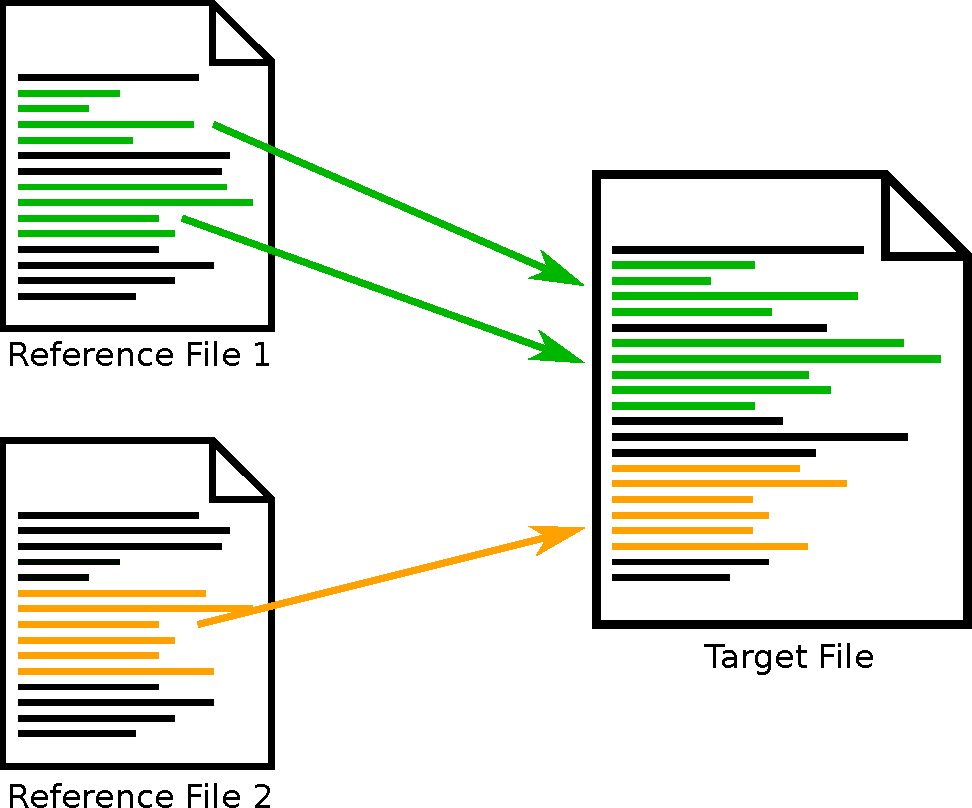
\includegraphics[width=0.8\linewidth]{figures/match_counting.pdf}
	\caption{Illustration of match counting}\label{fig:match_counting}
\end{figure}

\begin{table}[ht]
	\centering
	\newcolumntype{R}[1]{>{\raggedleft\arraybackslash}p{#1}}
	\begin{tabular}{l | l R{1cm} R{1cm} R{1cm}}
		& \textbf{Name} & \textbf{AC} & \textbf{OLC} & \textbf{LI} \\
		\hline 
		\parbox[t]{2mm}{\multirow{12}{*}{\rotatebox[origin=c]{90}{JAVA}}} 
		& IntelliJ IDEA Community & 0 & 0 & 0 \\
		& Eclipse JDT Core & 0 & 0 & 0 \\\
		& Elasticsearch & 0 & 0 & 0 \\
		& Eclipse JDT UI & 0 & 0 & 0 \\
		& Facebook Buck & 0 & 0 & 0 \\
		& Teamscale & 0 & 0 & 0 \\
		& Spring Boot & 0 & 0 & 0 \\
		& Openfire & 0 & 0 & 0 \\
		& Killbill & 0 & 0 & 0 \\
		& JabRef & 3 & 0 & 0 \\
		& Selenium & 0 & 0 & 0 \\
		& JUnit5 & 0 & 0 & 0 \\
		\hline 
		\parbox[t]{2mm}{\multirow{10}{*}{\rotatebox[origin=c]{90}{C/C++}}} 
		& Chromium & 0 & 0 & 0 \\
		& ArangoDB & 0 & 0 & 0 \\
		& Tensorflow & 0 & 0 & 0 \\
		& Apple Swift & 0 & 0 & 0 \\
		& Mesos & 0 & 0 & 0 \\
		& Apache httpd & 0 & 0 & 0 \\
		& RethinkDB & 0 & 0 & 0 \\
		& Tesseract & 0 & 0 & 0 \\
		& Bitcoin & 0 & 0 & 0 \\
		& Electron & 0 & 0 & 0 \\
	\end{tabular}
	\caption{Target projects and categorized matches}\label{table:scan_results}
\end{table}

The results show, that finding infringements is possible using this approach.
However, the amount of actual infringements in the detected copied code segments is rather small.
This is due to many accidental clones, which are caused by e.g. interface implementations or tables.

Otherwise licensed code which is copied sometimes is still a valid concern, since most licenses require to correctly attribute the source of the code.
In many cases, this is not done correctly, as manual inspection showed.
The violation of the license is still given in such a case, although it may not be as critical as e.g. with GPL licensed code.

\todo[inline]{attributed vs non-attributed (= violation) statistics}

\section{Special cases}
Some of the findings are rather special and can not be categorized precisely.
This section lists some of those cases and suggestions on how to handle those, if possible.

\begin{itemize}
	\item Overture -> Eclipse
	\item reverse copied code, e.g. Apache code in GPL
	\item Interface implementation quite similar: Java list implementation, equals code, tables in c
\end{itemize}

%\section{Database and Filter Sizes}
%The space $m$ in bits required to store $n$ values with the optimal number of hash functions can be estimated by \todo{quelle?}
%\begin{equation}\label{equ:bloom_probability} 
%m = -\frac{n\cdot \ln(p)}{(\ln2)^{2}}
%\end{equation}
%with $p$ being the probability for a false positive.
%For one billion hashes and a probability of 0.01\%, which roughly means one false positive for every 10000 lines of code, about 2,4 GB are needed.
%A simple hash table would need at least 16 GB for the same amount of data.
%TODO chunksize? => realtion to size of database

\section{Confidentiality}
The purpose of the tool proposed in this work is to uncover licensing issues and therefore may be used for closed source target systems.
One key issue for companies is confidentiality regarding own source code.
Uploading code to a server maintained externally to the company may not be conform with the company's data privacy policies.

The approach presented in this work is only sending hashes which encapsulate information relevant for identifying chunks.
In theory, this should restrict flow of information about the source code to a minimum and conclusions about the code can not be made.
However, when the code for a hash is known on the server side, i.e. a match for a hash is found, the server knows the code for the hash on the client.
If enough matches are found, the server may be able to reconstruct parts of the source code.
Still, information about the source code leaking from the client to the server is very limited.
\todo{Is this relevant? remove?}
\todo[inline]{further improve confidentiality: parital hashes}